\chapter{Interactions Between Species}\label{ch:b1:species-interactions}

In 1963, on a rocky shore of the Pacific, a young ecologist began
throwing every starfish he found on a stretch of rock back into the
sea, and kept doing it for years. The starfish ate mussels. Without
them, the mussels spread downward over the rock and crowded out the
barnacles, limpets, chitons and algae that had lived there; a
\omterm{def:b1:ecosystem-organization:ecosystem}{community} of fifteen species fell to eight. One predator, itself
neither abundant nor large, had been holding the whole assembly in
place. Species do not merely share a place; they compete for it, eat
one another, live inside and upon one another, and depend on one
another, and the \omterm{def:b1:ecosystem-organization:ecosystem}{community} is the sum of these interactions. This
chapter classifies them, gives the quantitative models of \omterm{def:b1:species-interactions:types}{competition}
and \omterm{def:b1:species-interactions:types}{predation} that a first year can handle, and shows through
experiments how one interaction can shape a whole \omterm{def:b1:ecosystem-organization:ecosystem}{ecosystem}.

\section{A classification of interactions}

\begin{definition}[Interspecific interactions]\label{def:b1:species-interactions:types}
\index{competition}\index{predation}\index{parasitism}\index{mutualism}\index{commensalism}
An interaction between two species is classified by its effect on
each: $+$ (benefit), $-$ (harm) or $0$. \emph{Competition} ($-/-$): both
use a resource in short supply. \emph{Predation} ($+/-$): one kills
and eats the other; \emph{herbivory} ($+/-$) when the eaten is a plant
and usually survives; \emph{parasitism} ($+/-$) when the exploiter
lives on or in a host it does not kill at once. \emph{Mutualism}
($+/+$): both benefit. \emph{Commensalism} ($+/0$): one benefits, the
other is unaffected. \emph{Amensalism} ($-/0$): one is harmed, the
other unaffected. Every interaction is a selective pressure on both
partners, and their reciprocal adaptation over generations is
\emph{coevolution}.
\end{definition}

\begin{example}[One tree, all six]\label{ex:b1:species-interactions:oak}
An oak competes with its neighbours for light; its acorns are eaten by
jays (\omterm{def:b1:species-interactions:types}{predation}) and its \omterm{def:b1:flowering-plant-organization:organs}{leaves} by caterpillars (herbivory); mistletoe
draws its sap (\omterm{def:b1:species-interactions:types}{parasitism}); its \omterm{def:b1:flowering-plant-organization:organs}{roots} exchange sugars for phosphate
with a fungus (\omterm{def:b1:species-interactions:types}{mutualism}); ferns grow on its bark, using it only as a
perch (\omterm{def:b1:species-interactions:types}{commensalism}); and its shade kills the grass beneath it
(amensalism).
\end{example}

\section{Competition}

\begin{definition}[Interspecific competition]\label{def:b1:species-interactions:competition}
\index{competitive exclusion}\index{niche partitioning}\index{character displacement}
Two species compete when they both use a resource --- food, light,
water, space, nesting sites --- whose supply limits their growth.
\omterm{def:b1:species-interactions:types}{Competition} may be by \emph{exploitation} (each takes what the other
would have used) or by \emph{interference} (direct aggression, toxins,
territories). Its outcome follows the \emph{competitive exclusion
principle}: two species that need the same limiting resource in the
same way cannot coexist indefinitely in a stable environment; the
better competitor eliminates the other. Coexisting competitors
therefore differ in \omterm{def:b1:ecosystem-organization:niche}{niche} (\emph{\omterm{def:b1:ecosystem-organization:niche}{niche} partitioning}) --- and where two
species overlap they often diverge in form more than where each lives
alone (\emph{character displacement}).
\end{definition}

\begin{proposition}[The Lotka--Volterra competition model]\label{prop:b1:species-interactions:lotka}
Let two species grow logistically (\cref{ch:b1:populations}) and let
each individual of species 2 count as $\alpha$ individuals of species
1 in the use of species 1's resource, and each of species 1 as $\beta$
of species 2:
\[
\frac{\dd N_1}{\dd t} = r_1 N_1\left(1 - \frac{N_1 + \alpha N_2}{K_1}\right),
\qquad
\frac{\dd N_2}{\dd t} = r_2 N_2\left(1 - \frac{N_2 + \beta N_1}{K_2}\right).
\]
Species 1 stops growing on the line $N_1 + \alpha N_2 = K_1$ (its
\emph{isocline}\index{isocline}), species 2 on $N_2 + \beta N_1 = K_2$. If
each species limits itself more than it limits the other ($\alpha <
K_1/K_2$ and $\beta < K_2/K_1$) the \omterm{prop:b1:species-interactions:lotka}{isoclines} cross with both species'
equilibrium stable and they \emph{coexist}; if one \omterm{prop:b1:species-interactions:lotka}{isocline} lies
entirely above the other, that species always \emph{excludes} the
other; if each limits the other more than itself, the winner depends
on the starting numbers.
\end{proposition}
\begin{proof}[Partial proof]
Species 1 grows below its \omterm{prop:b1:species-interactions:lotka}{isocline} and declines above it; species 2
likewise. When the \omterm{prop:b1:species-interactions:lotka}{isoclines} cross with species 1's above species
2's on the $N_1$ axis and below it on the $N_2$ axis, a point off the
crossing is pushed back toward it from every side: the crossing is a
stable equilibrium with both species present. When species 1's
\omterm{prop:b1:species-interactions:lotka}{isocline} lies entirely outside species 2's, every point where species
2 could still grow is also a point where species 1 grows and it goes
on growing after species 2 has stopped, until it reaches $K_1$ with
$N_2 = 0$. The full analysis is done in the Year 2 volume; the sketch
of the \omterm{prop:b1:species-interactions:lotka}{isoclines} gives every outcome without it.
\end{proof}

\begin{omfigure}
\begin{tikzpicture}[font=\footnotesize, >=Stealth, line cap=round]
  \begin{scope}
    \draw[->, thick] (0,0) -- (4.6,0) node[below left] {$N_1$};
    \draw[->, thick] (0,0) -- (0,4.4) node[below right] {$N_2$};
    \draw[very thick, omDef] (4.0,0) -- (0,3.0) node[pos=0.15, above right, omDef!80!black] {species 1 stops};
    \draw[very thick, omThm] (2.6,0) -- (0,4.0) node[pos=0.85, right, omThm!80!black] {species 2 stops};
    \fill (1.63,1.78) circle (2pt); \node[anchor=west] at (1.75,1.95) {stable coexistence};
    \draw[->, gray] (3.6,3.0) -- (2.2,2.2); \draw[->, gray] (0.4,0.4) -- (1.3,1.4);
    \node[anchor=north] at (2.3,-0.8) {each species limits itself more};
  \end{scope}
  \begin{scope}[xshift=7.2cm]
    \draw[->, thick] (0,0) -- (4.6,0) node[below left] {$N_1$};
    \draw[->, thick] (0,0) -- (0,4.4) node[below right] {$N_2$};
    \draw[very thick, omDef] (4.0,0) -- (0,4.0) node[pos=0.5, above right, omDef!80!black] {species 1 stops};
    \draw[very thick, omThm] (2.4,0) -- (0,2.4) node[pos=0.35, anchor=north east, align=right, omThm!80!black] {species 2\\ stops};
    \fill (4.0,0) circle (2pt); \node[anchor=north, font=\scriptsize] at (3.5,-0.3) {species 1 alone at $K_1$};
    \draw[->, gray] (1.0,3.4) -- (2.1,2.3); \draw[->, gray] (2.4,2.0) -- (3.4,0.7);
    \node[anchor=north] at (2.3,-0.8) {species 1 wins everywhere};
  \end{scope}
\end{tikzpicture}

{\small Two outcomes of two-species \omterm{def:b1:species-interactions:types}{competition}, read from the
\omterm{prop:b1:species-interactions:lotka}{isoclines} (the lines where each species stops growing). Left: the
\omterm{prop:b1:species-interactions:lotka}{isoclines} cross so that each species is held back more by itself
than by the other, and they coexist. Right: species 1's \omterm{prop:b1:species-interactions:lotka}{isocline}
lies outside species 2's, and species 1 always wins.}
\end{omfigure}

\begin{proposition}[Competitive exclusion]\label{prop:b1:species-interactions:gause}
\index{Gause's principle}
Two species competing for one limiting resource in a constant
environment cannot both persist: the one whose \omterm{def:b1:populations:population}{population} can keep
growing at the lower resource level drives the resource below what
the other needs, and the other declines to extinction.
\end{proposition}
\begin{proof}[Evidence]
Gause (1934) grew two ciliates, \emph{Paramecium aurelia} and
\emph{P.~caudatum}, on a daily ration of bacteria. Alone, each grew
logistically to its own plateau. Together, \emph{P.~aurelia}, which
grows faster and needs less food per individual, reached nearly its
plateau while \emph{P.~caudatum} declined to nothing within sixteen
days. A third species, \emph{P.~bursaria}, which feeds at the bottom
of the tube where \emph{P.~aurelia} does not, coexisted with it
indefinitely: the exclusion held only when the \omterm{def:b1:ecosystem-organization:niche}{niches} were the same.
\end{proof}

\begin{omfigure}
\begin{tikzpicture}
\begin{axis}[
  width=0.8\linewidth, height=6.2cm,
  axis x line=bottom, axis y line=left,
  xmin=0, xmax=20, ymin=0, ymax=220,
  xlabel={days}, ylabel={individuals per \qty{0.5}{mL}},
  xlabel style={font=\small}, ylabel style={font=\small},
  tick label style={font=\small},
  legend style={font=\scriptsize, at={(0.98,0.02)}, anchor=south east, draw=none, fill=none},
  legend cell align=left,
]
\addplot[omDef, very thick, dashed, domain=0:20, samples=60] {200/(1+40*exp(-0.8*x))};
\addlegendentry{\emph{P.~aurelia} alone}
\addplot[omThm, very thick, dashed, domain=0:20, samples=60] {130/(1+25*exp(-0.55*x))};
\addlegendentry{\emph{P.~caudatum} alone}
\addplot[omDef, very thick, domain=0:20, samples=60] {170/(1+40*exp(-0.65*x))};
\addlegendentry{\emph{P.~aurelia} mixed}
\addplot[omThm, very thick, domain=0:20, samples=80] {80*exp(-0.05*(x-6)^2)*(x<12) + 80*exp(-0.05*36)*exp(-0.5*(x-12))*(x>=12)};
\addlegendentry{\emph{P.~caudatum} mixed}
\end{axis}
\end{tikzpicture}

{\small Gause's \omterm{def:b1:species-interactions:types}{competition} experiment (redrawn from his data).
Each species alone grows to its plateau; together, \emph{P.~aurelia}
rises almost to its own while \emph{P.~caudatum} peaks and is driven
to extinction.}
\end{omfigure}

\begin{example}[Character displacement in finches]\label{ex:b1:species-interactions:finches}
On islands where a single ground finch lives alone its beak is of
middle size; where two species share an island their beaks are
respectively smaller and larger than either has alone, each species
having shifted toward seeds the other cannot crack. The \omterm{def:b1:ecosystem-organization:niche}{niches} were
partitioned by evolution, and the partition is visible in the beak.
\end{example}

\section{Predation and herbivory}

\begin{definition}[Functional response]\label{def:b1:species-interactions:functional}
\index{functional response}\index{handling time}
The \emph{functional response} of a predator is the number of prey
one predator eats per unit time as a function of prey density $N$.
\emph{Type I}: proportional to $N$ (a filter-feeder). \emph{Type II}:
rises then saturates, because each prey takes a \emph{handling time}
$h$ to catch, eat and digest, during which no other can be taken.
\emph{Type III}: sigmoid --- low at low density because the predator
ignores or cannot find rare prey, then rising steeply (a predator that
switches to whatever is common). The \emph{numerical response} is the
change in the number of predators with prey density, through
reproduction or immigration.
\end{definition}

\begin{theorem}[The disc equation]\label{thm:b1:species-interactions:holling}
\index{disc equation}
If a predator searches at an \emph{attack rate} $a$ (area swept per
unit time, times the probability of capture) and spends a \omterm{def:b1:species-interactions:functional}{handling
time} $h$ on each prey, the number of prey taken per predator per unit
time at prey density $N$ is
\[
f(N) = \frac{aN}{1 + ahN} ,
\]
rising linearly as $aN$ at low density and saturating at $1/h$ at
high density; $f$ is half its maximum when $N = 1/(ah)$. In the form
$1/f = 1/(aN) + h$ a plot of $1/f$ against $1/N$ is a straight line
of slope $1/a$ and intercept $h$.
\end{theorem}
\begin{proof}
Over a total time $T$ the predator searches for $T_s$ and handles for
the rest. Searching, it encounters prey at rate $aN$, so the number
caught is $n = aN T_s$; handling them takes $nh$, so $T = T_s + nh =
n/(aN) + nh$, whence $n/T = aN/(1 + ahN)$. When $ahN \ll 1$ handling is
negligible and $f \approx aN$; when $ahN \gg 1$ the predator does
nothing but handle and $f \to 1/h$. Inverting gives the linear form.
\end{proof}
\begin{proof}[Evidence]
Holling (1959) had a blindfolded assistant ``prey'' with a fingertip
on sandpaper discs scattered on a table, picking up each found disc
(the \omterm{def:b1:species-interactions:functional}{handling time}) before searching again; the number found per
minute against disc density gave exactly this curve, and the equation
took its name from the experiment. Real predators --- a mantis on
flies, a stickleback on water fleas --- give the same shape, with
\omterm{def:b1:species-interactions:functional}{handling times} of seconds to hours.
\end{proof}

\begin{omfigure}
\begin{tikzpicture}
\begin{axis}[
  width=0.78\linewidth, height=6.2cm,
  axis x line=bottom, axis y line=left,
  xmin=0, xmax=100, ymin=0, ymax=12,
  xlabel={prey density $N$ (per \unit{m^2})}, ylabel={prey eaten per predator per day},
  xlabel style={font=\small}, ylabel style={font=\small},
  tick label style={font=\small},
  legend style={font=\scriptsize, at={(0.98,0.03)}, anchor=south east, draw=none, fill=none},
  legend cell align=left,
]
\addplot[omExo!80!black, very thick, domain=0:100, samples=2] {0.1*x};
\addlegendentry{type I: $f = aN$}
\addplot[omDef, very thick, domain=0:100, samples=80] {0.5*x/(1+0.05*x)};
\addlegendentry{type II: $f = aN/(1+ahN)$, plateau $1/h = 10$}
\addplot[omThm, very thick, domain=0:100, samples=80] {10*x^2/(30^2+x^2)};
\addlegendentry{type III: sigmoid}
\draw[dashed, gray] (axis cs:0,10) -- (axis cs:100,10);
\end{axis}
\end{tikzpicture}

{\small The three \omterm{def:b1:species-interactions:functional}{functional responses}. Type II saturates at $1/h$
(here ten prey a day, a \omterm{def:b1:species-interactions:functional}{handling time} of \qty{2.4}{h}); type III
starts slowly because rare prey are overlooked.}
\end{omfigure}

\begin{proposition}[Defences and the arms race]\label{prop:b1:species-interactions:defences}
\index{mimicry}\index{aposematism}
Prey and plants evolve defences --- crypsis, armour, spines, speed,
toxins and their warning colours (\emph{aposematism}), and
\emph{mimicry}: a harmless species copying a toxic one (Batesian) or
several toxic species converging on one pattern (Müllerian). Plants
defend themselves with thorns, silica, tannins, alkaloids and
cyanogenic glycosides, often induced by damage. Predators and
herbivores evolve counter-measures --- keener senses, detoxifying
\omterm{def:b1:enzymes:enzyme}{enzymes}, resistance to the toxin --- and the pair coevolve. The
result is not the destruction of the prey but a running balance: a
predator that ate its prey to extinction would follow it.
\end{proposition}

\begin{omfigure}
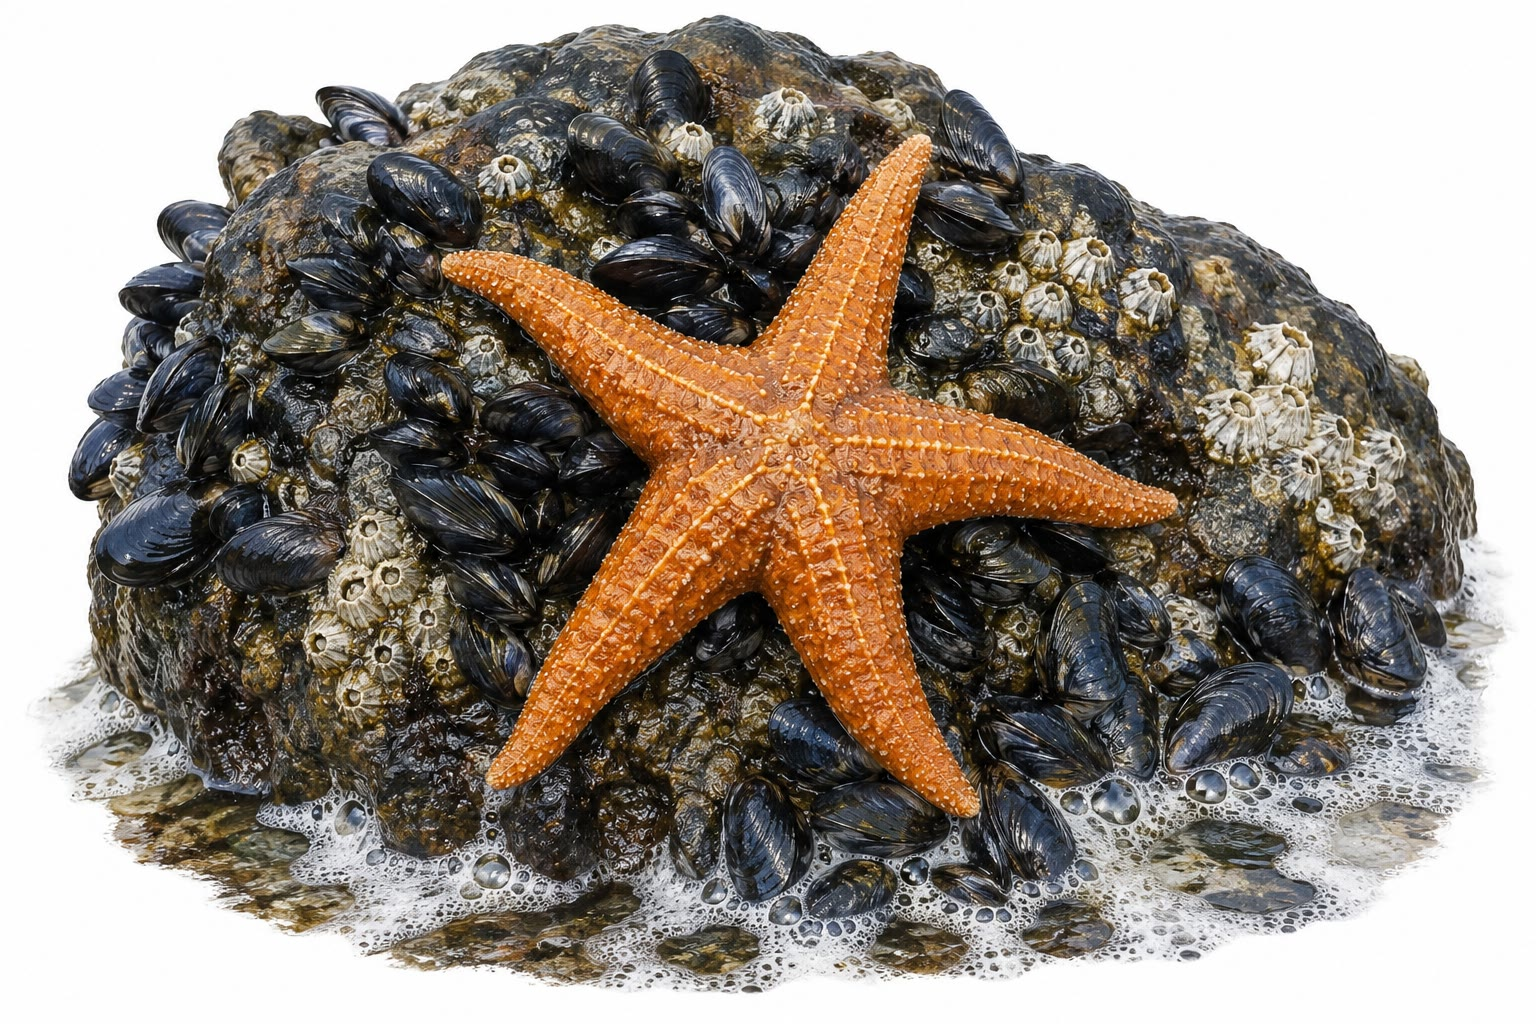
\includegraphics[width=0.6\linewidth]{images/book3/ai/b3-27-sea-star-mussels.jpg}

{\small A predatory sea star on a mussel bed at low tide: the
keystone predator whose removal turned a fifteen-species shore into
a mussel monoculture.}
\end{omfigure}

\section{Living together: parasitism, mutualism, commensalism}

\begin{definition}[Parasitism, symbiosis, mutualism]\label{def:b1:species-interactions:symbiosis}
\index{symbiosis}\index{parasite}\index{lichen}
A \emph{parasite} lives at the expense of a host, on it (ectoparasite:
tick, louse, mistletoe) or in it (endoparasite: tapeworm, malaria
parasite, rust fungus), taking nutrients and reducing its fitness
without necessarily killing it; parasites are often specialised,
with complex life cycles through several hosts. A \emph{symbiosis} is
any close, lasting association between two species; a \emph{\omterm{def:b1:species-interactions:types}{mutualism}}
is one that benefits both: the \omterm{def:b1:plant-water-minerals:mycorrhiza}{mycorrhiza} (a fungus on or in
plant \omterm{def:b1:flowering-plant-organization:organs}{roots}, exchanging phosphate and water for sugar;
\cref{ch:b1:plant-water-minerals}), the \omterm{def:b1:plant-water-minerals:nodules}{root nodule} (nitrogen-fixing
bacteria fed by the legume), the \emph{lichen} (a fungus housing an
alga or cyanobacterium), the reef coral (a cnidarian housing
photosynthetic dinoflagellates), the gut microbiota of a ruminant or
a termite (\cref{ch:b1:digestion-absorption}), and pollination (nectar
for pollen transport). Many \omterm{def:b1:species-interactions:types}{mutualisms} began as \omterm{def:b1:species-interactions:types}{parasitisms} or
\omterm{def:b1:species-interactions:types}{predations} that the partners' coevolution turned to mutual benefit,
and remain conditional: a mycorrhizal fungus in a phosphate-rich soil
is a cost, and the plant reduces it.
\end{definition}

\begin{example}[Pollination as a trade]\label{ex:b1:species-interactions:pollination}
A flower spends a few joules of sugar on nectar; a bee spends flight
to collect it and carries pollen between flowers as it goes. The
flower's colour, scent, shape and timing are addressed to its
pollinators, and the bee's tongue length, colour vision and foraging
memory to its flowers; some pairs are so tightly fitted --- a long
nectar spur and the one moth whose tongue reaches it --- that neither
survives without the other, and a whole plant \omterm{def:b1:ecosystem-organization:ecosystem}{community} can depend on
a few species of insect.
\end{example}

\begin{omfigure}
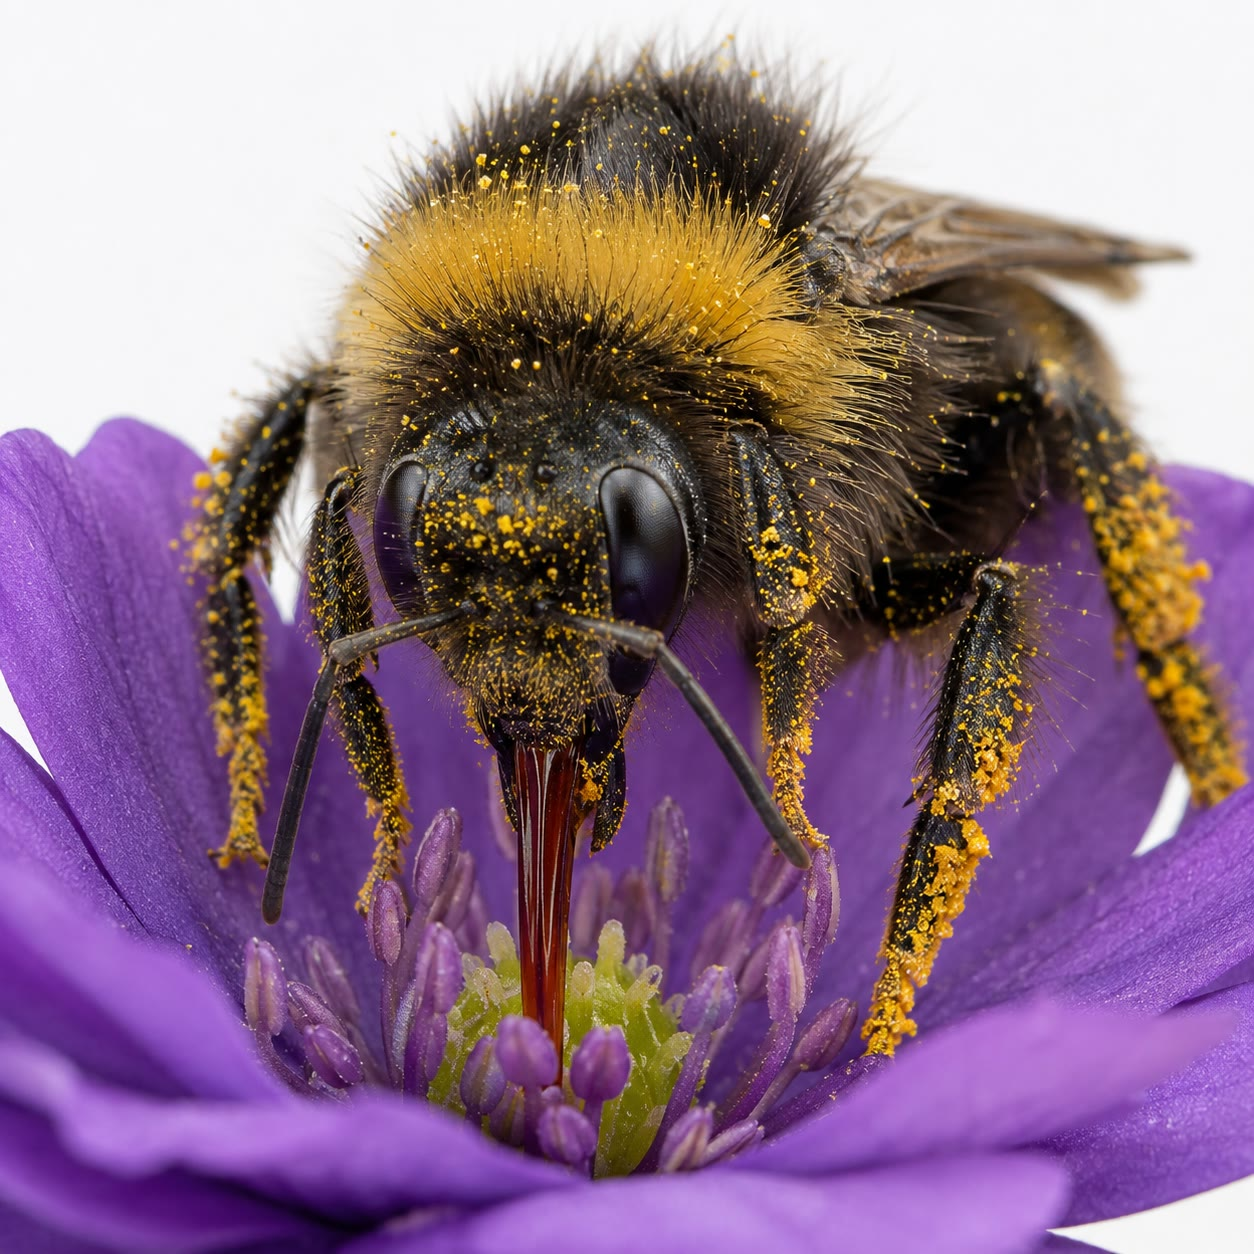
\includegraphics[width=0.56\linewidth]{images/book3/ai/b3-27-bee-flower.jpg}

{\small A \omterm{def:b1:species-interactions:types}{mutualism} at work: nectar for the bee, pollen transport for
the flower. Each partner's form has been shaped by the other.}
\end{omfigure}

\begin{remark}[Commensalism is rare and unstable]\label{rem:b1:species-interactions:commensal}
Few interactions are truly $+/0$: the epiphyte that shades its host,
the remora that costs its shark a little drag, the cattle egret that
eats what the cattle stir up are commensals only to the precision of
the measurement. Interactions are classified by their net effect, and
the net effect can change with conditions.
\end{remark}

\section{Interactions that shape the community}

\begin{definition}[Keystone species, trophic cascade]\label{def:b1:species-interactions:keystone}
\index{keystone species}\index{trophic cascade}
A \emph{keystone species} is one whose effect on the \omterm{def:b1:ecosystem-organization:ecosystem}{community} is out
of proportion to its abundance or biomass: remove it and the
\omterm{def:b1:ecosystem-organization:ecosystem}{community}'s structure changes, usually because it controls a dominant
competitor. A \emph{trophic cascade} is the propagation of an effect
down a \omterm{def:b1:ecosystem-organization:foodweb}{food chain} across more than one level: a predator's presence
lowers the herbivores, which raises the plants; its removal does the
reverse. Cascades show that \omterm{def:b1:ecosystem-organization:ecosystem}{communities} are structured from the top as
well as from the bottom (by productivity, \cref{ch:b1:ecosystem-organization}).
\end{definition}

\begin{proposition}[A predator can maintain diversity]\label{prop:b1:species-interactions:paine}
By eating the species that would otherwise win the \omterm{def:b1:species-interactions:types}{competition} for
space or resources, a predator keeps the losers in the \omterm{def:b1:ecosystem-organization:ecosystem}{community}; its
removal lets the dominant competitor exclude them, and diversity
falls.
\end{proposition}
\begin{proof}[Evidence]
Paine (1966) removed the sea star \emph{Pisaster} from an
\qty{8}{m} stretch of rocky shore on the Pacific coast of North
America and left a neighbouring stretch as control. The sea star eats
mussels, barnacles and other sessile animals, mussels by preference.
Within two years the mussel \emph{Mytilus} had spread down the rock
and taken nearly all the space; the barnacles, chitons, limpets and
algae that had lived in the gaps disappeared, and the fifteen
species of the control plot fell to eight. The predator's own share of
the \omterm{def:b1:ecosystem-organization:ecosystem}{community}'s biomass was small; its removal changed everything.
\end{proof}

\begin{omfigure}
\begin{tikzpicture}
\begin{axis}[
  width=0.74\linewidth, height=5.6cm,
  axis x line=bottom, axis y line=left,
  xmin=1963, xmax=1969, ymin=0, ymax=18,
  xlabel={year}, ylabel={species on the plot},
  xlabel style={font=\small}, ylabel style={font=\small},
  tick label style={font=\small}, xtick={1963,1964,1965,1966,1967,1968},
  x tick label style={/pgf/number format/1000 sep=},
  legend style={font=\scriptsize, at={(0.98,0.03)}, anchor=south east, draw=none, fill=none},
  legend cell align=left,
]
\addplot[omDef, very thick, mark=*] coordinates {(1963,15) (1964,15) (1965,14) (1966,15) (1967,15) (1968,15)};
\addlegendentry{control: sea star present}
\addplot[omThm, very thick, mark=square*] coordinates {(1963,15) (1964,12) (1965,10) (1966,9) (1967,8) (1968,8)};
\addlegendentry{sea star removed}
\node[font=\scriptsize, anchor=south west, align=left] at (axis cs:1966.2,10.6) {mussels take\\ the rock};
\end{axis}
\end{tikzpicture}

{\small Paine's removal experiment (after his data). Diversity on the
plot without the predator falls by half in five years while the
control keeps its fifteen species.}
\end{omfigure}

\begin{example}[Wolves, elk and willows]\label{ex:b1:species-interactions:wolves}
Wolves were exterminated from a large mountain park in the 1920s;
its elk multiplied and browsed the willows and aspens along the
rivers to stubs; beavers, which need willow, dwindled; songbirds lost
their thickets. When wolves were reintroduced in 1995 the elk
declined and, more important, avoided the valley bottoms where they
were vulnerable; the willows regrew, beavers returned and built dams,
and the wetlands they made brought back fish, amphibians and birds.
The cascade ran from a carnivore through a herbivore to the plants
and from there to a dozen species that never met a wolf --- with
weather, hunting and other predators contributing, so that the
wolves' share of the change is still debated.
\end{example}

\begin{omfigure}
\begin{tikzpicture}[font=\footnotesize, >=Stealth, line cap=round,
  lv/.style={draw, thick, rounded corners=3pt, inner sep=4pt, align=center, fill=white, minimum width=2.6cm}]
  \node[lv, fill=omDef!25] (wolf) at (0,4.5) {wolves};
  \node[lv, fill=omProp!20] (elk) at (0,2.8) {elk};
  \node[lv, fill=omExo!20] (willow) at (0,1.1) {willows, aspens};
  \node[lv, fill=omProp!20] (beaver) at (3.8,1.1) {beavers};
  \node[lv, fill=omDef!12] (wet) at (7.4,1.1) {ponds, wetlands};
  \node[lv, fill=omThm!15] (birds) at (3.8,-0.6) {songbirds, fish,\\ amphibians};
  \draw[->, very thick, omThm] (wolf) -- (elk) node[midway, right] {$-$: fewer, and kept off the river banks};
  \draw[->, very thick, omThm] (elk) -- (willow) node[midway, left] {$-$: browsing};
  \draw[->, very thick, omDef] (willow) -- (beaver) node[midway, above=9pt] {$+$: food, dams};
  \draw[->, very thick, omDef] (beaver) -- (wet) node[midway, above] {$+$};
  \draw[->, very thick, omDef] (willow) -- (birds) node[midway, below left] {$+$};
  \draw[->, very thick, omDef] (wet) |- (birds) node[pos=0.8, below] {$+$};
  \node[anchor=north, align=center, gray] at (3.4,-1.5) {two minus signs make a plus: the wolves' return increased the willows,\\ and the willows carried the effect to species the wolves never touched};
\end{tikzpicture}

{\small A \omterm{def:b1:species-interactions:keystone}{trophic cascade}: an effect passing down three levels and
sideways through the \omterm{def:b1:ecosystem-organization:ecosystem}{community}. Signs give the direction of each
link.}
\end{omfigure}

\begin{omfigure}
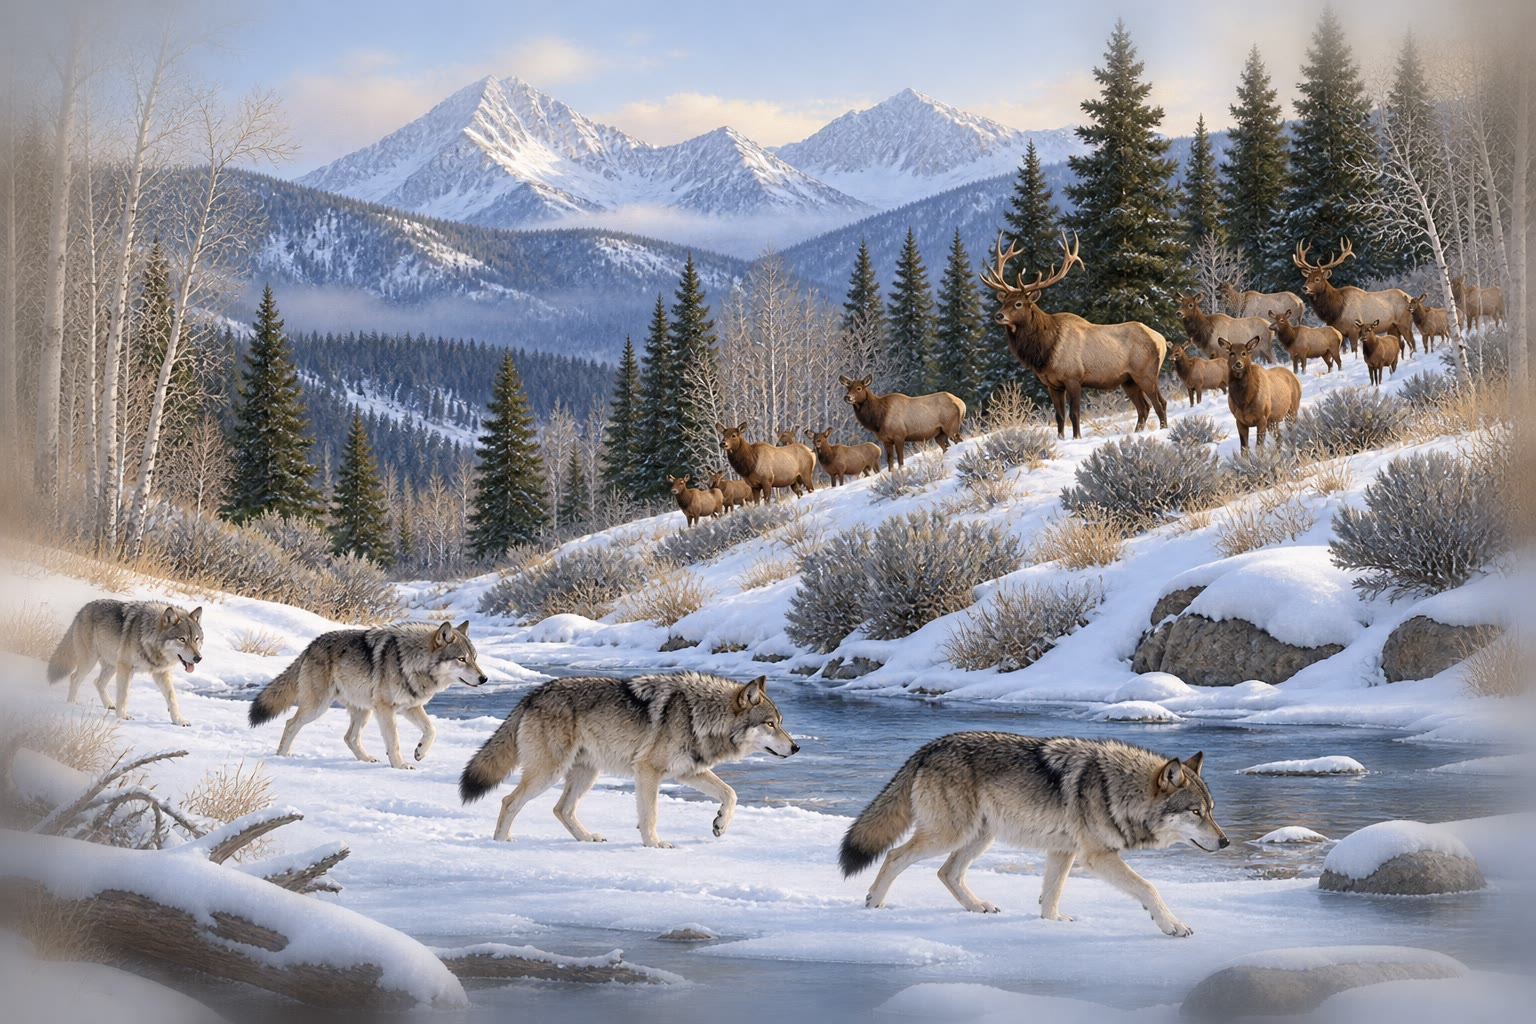
\includegraphics[width=0.6\linewidth]{images/book3/ai/b3-27-wolves-elk.jpg}

{\small Wolves and elk in a river valley in winter. The predator's
effect on the vegetation runs through where the elk dare to graze as
much as through how many of them there are.}
\end{omfigure}

\begin{method}[Reading an interaction from an experiment]\label{met:b1:species-interactions:reading}
\begin{enumerate}
  \item Identify the manipulation (removal, addition, exclusion cage,
        pairing in culture) and the control kept alongside it under
        the same conditions.
  \item For each species, compare its abundance with and without the
        partner: the sign of the difference gives the sign of the
        interaction on that species.
  \item Look for indirect effects: a species that changed without
        touching the manipulated one is at the end of a chain ---
        find the intermediates.
  \item Check the time scale (a \omterm{def:b1:species-interactions:types}{competition} can take many generations
        to resolve; a cascade runs at the rate of the slowest level)
        and the spatial scale (does the result hold beyond the plot?).
  \item Fit the model where the data allow: logistic curves and
        \omterm{prop:b1:species-interactions:lotka}{isoclines} for \omterm{def:b1:species-interactions:types}{competition}, the \omterm{thm:b1:species-interactions:holling}{disc equation} for a \omterm{def:b1:species-interactions:functional}{functional
        response}, and read the parameters off the linearised plots.
\end{enumerate}
\end{method}

\section{Exercises}

\begin{exercise}[$\star$]\label{exo:b1:species-interactions:1}
Give the sign pair and an example for each of the six kinds of
interaction.
\end{exercise}

\begin{exercise}[$\star$]\label{exo:b1:species-interactions:2}
State the \omterm{def:b1:species-interactions:competition}{competitive exclusion} principle and say why it does not
forbid five warblers in one spruce.
\end{exercise}

\begin{exercise}[$\star$]\label{exo:b1:species-interactions:3}
Define \omterm{def:b1:species-interactions:functional}{handling time} and attack rate, and give the maximum feeding
rate of a predator with $h = \qty{30}{min}$.
\end{exercise}

\begin{exercise}[$\star$]\label{exo:b1:species-interactions:4}
What is a \omterm{def:b1:species-interactions:keystone}{keystone species}? Why is a \omterm{def:b1:species-interactions:keystone}{keystone species} not simply the
most abundant one?
\end{exercise}

\begin{exercise}[$\star\star$]\label{exo:b1:species-interactions:5}
Species 1 has $K_1 = 500$, species 2 has $K_2 = 400$, with $\alpha =
0.5$ and $\beta = 0.6$. Draw the \omterm{prop:b1:species-interactions:lotka}{isoclines} and give the outcome.
Repeat with $\alpha = 2$, $\beta = 0.6$.
\end{exercise}

\begin{exercise}[$\star\star$]\label{exo:b1:species-interactions:6}
A predator with $a = \qty{0.2}{m^2/h}$ and $h = \qty{0.25}{h}$ meets
prey at \qty{10}{} and \qty{100}{} per square metre. Compute its
feeding rate in each case and the density at which it is half
saturated.
\end{exercise}

\begin{exercise}[$\star\star$]\label{exo:b1:species-interactions:7}
Why does a type III response stabilise a prey \omterm{def:b1:populations:population}{population} at low
density while a type II does not?
\end{exercise}

\begin{exercise}[$\star\star$]\label{exo:b1:species-interactions:8}
From Gause's experiment, explain why \emph{P.~bursaria} coexisted
with \emph{P.~aurelia} but \emph{P.~caudatum} did not. What made the
difference: growth rate or \omterm{def:b1:ecosystem-organization:niche}{niche}?
\end{exercise}

\begin{exercise}[$\star\star$]\label{exo:b1:species-interactions:9}
A Batesian mimic becomes more common than its toxic model. Predict
what happens to the protection of both, and why the mimic's success
is self-limiting.
\end{exercise}

\begin{exercise}[$\star\star\star$]\label{exo:b1:species-interactions:10}
Paine's removal plot lost seven species. Explain, using the \omterm{prop:b1:species-interactions:lotka}{isocline}
model, how a predator that eats the dominant competitor converts an
exclusion into a coexistence.
\end{exercise}

\begin{exercise}[$\star\star\star$]\label{exo:b1:species-interactions:11}
A mycorrhizal fungus takes \qty{15}{\%} of a plant's photosynthate and
supplies \qty{80}{\%} of its phosphate. In what conditions is the
association a \omterm{def:b1:species-interactions:types}{mutualism}, and in what conditions a \omterm{def:b1:species-interactions:types}{parasitism}? Propose
an experiment to tell.
\end{exercise}

\begin{exercise}[$\star\star\star$]\label{exo:b1:species-interactions:12}
Design an experiment to test whether the wolves, rather than the
weather or hunting, caused the willows' recovery: controls, replicates,
the variables to measure, and what result would refute the cascade.
\end{exercise}

\section{Problem: The Predator and the Shore}

\begin{problem}[{Weekend problem --- Gause's ciliates in a tube, a
predator's feeding data fitted to the disc equation, Paine's shore
with and without its sea star, and a pollinator's budget, ending on the
attack rate and handling time of the predator}]
\label{pb:b1:species-interactions:1}

\medskip
\noindent\textbf{Part I --- \omterm{def:b1:species-interactions:types}{Competition} in a tube.}
Two ciliates are grown alone: species A reaches $K_A = 200$ per
\qty{0.5}{mL} with $r_A = \qty{0.8}{d^{-1}}$; species B reaches
$K_B = 130$ with $r_B = \qty{0.55}{d^{-1}}$. Together, an individual
of B uses as much food as $\alpha = 1.4$ of A, and an individual of A
as much as $\beta = 0.9$ of B.
\begin{enumerate}
  \item Write the two \omterm{prop:b1:species-interactions:lotka}{isoclines} and their intercepts on the axes.
  \item Draw them and state which species wins, and why the outcome
        does not depend on the starting numbers.
  \item From the doubling times ($\ln 2/r$), which species would you
        have expected to win from growth rate alone?
  \item A third species C feeds on the bottom of the tube and competes
        with A only weakly ($\alpha = 0.3$, $\beta = 0.3$, $K_C = 100$).
        Draw the \omterm{prop:b1:species-interactions:lotka}{isoclines} and give the outcome.
  \item Why does the exclusion principle hold in a tube and so often
        fail in a forest? Give two reasons.
  \item Compute the equilibrium numbers of A and C from the crossing of
        the \omterm{prop:b1:species-interactions:lotka}{isoclines}.
\end{enumerate}

\medskip
\noindent\textbf{Part II --- The \omterm{thm:b1:species-interactions:holling}{disc equation}.}
A predatory beetle is offered prey at densities of 5, 10, 20, 40 and
80 per square metre; it eats 2.0, 3.3, 5.0, 6.7 and 8.0 prey per day
respectively.
\begin{enumerate}[resume]
  \item Plot the feeding rate against density and identify the type of
        response.
  \item Compute $1/f$ and $1/N$ for each point and plot them.
  \item From the slope and intercept, obtain $a$ and $h$.
  \item Compute the maximum feeding rate and the half-saturation
        density.
  \item At which of the five densities does the beetle spend more
        than half its time handling?
  \item The beetle's prey grow logistically with $r = \qty{0.1}{d^{-1}}$
        and $K = 200$. At what density is the prey's growth (per
        beetle-free square metre) equal to the beetle's consumption if
        there is one beetle per square metre? Is this equilibrium
        stable against a small rise in prey?
  \item A second prey species appears that the beetle handles twice as
        fast. Predict the change in the beetle's total intake at high
        density.
\end{enumerate}

\medskip
\noindent\textbf{Part III --- The shore.}
On Paine's control plot the \omterm{def:b1:ecosystem-organization:ecosystem}{community} had 15 species; on the removal
plot the count fell 15, 12, 10, 9, 8, 8 over five years, and the
mussels' cover of the rock rose from \qty{20}{\%} to \qty{85}{\%}.
\begin{enumerate}[resume]
  \item Compute the \omterm{def:b1:ecosystem-organization:diversity}{Shannon index} of a plot with 15 species at equal
        abundance, and of one with 8 species where mussels are
        \qty{85}{\%} of individuals and the other seven share the rest
        equally.
  \item By what factor did the diversity fall?
  \item Explain, with the signs of the interactions, why removing a
        $+/-$ interaction (\omterm{def:b1:species-interactions:types}{predation} on mussels) strengthened a $-/-$
        one (\omterm{def:b1:species-interactions:types}{competition} for rock).
  \item The sea star was less than \qty{1}{\%} of the plot's biomass.
        Why is biomass a poor guide to a species' importance?
  \item Predict what would have happened had the sea star's preferred
        prey been the rarest species rather than the dominant one.
  \item Propose a way to confirm that it was \omterm{def:b1:species-interactions:types}{predation} on mussels and
        not some other effect of the sea star (a caging experiment).
\end{enumerate}

\medskip
\noindent\textbf{Part IV --- A \omterm{def:b1:species-interactions:types}{mutualism}'s budget.}
A bee visits 1000 flowers in a day and collects \qty{40}{mg} of sugar;
each flower gives \qty{40}{\micro g} of sugar in nectar and receives
pollen from, on average, 3 previous flowers per visit. The plant
spends \qty{1}{\%} of its daily photosynthate (\qty{4}{mg} of sugar per
flower) on nectar; a bee's flight costs \qty{0.5}{mg} of sugar per
hour of foraging (\qty{8}{h}).
\begin{enumerate}[resume]
  \item Compute the bee's net daily gain of sugar and its energy
        equivalent at \qty{16}{kJ/g}.
  \item Compute the plant's daily cost per flower as a fraction of its
        photosynthate and say what it buys.
  \item Why is this interaction $+/+$ even though each partner is
        exploiting the other?
  \item A nectar robber bites the base of the flower and takes the
        nectar without touching the pollen. Give the signs of the
        robber--plant interaction and its likely effect on the bee.
  \item Draw the sign diagram of plant, bee, robber and a bird that
        eats robbers, and predict the bird's indirect effect on the
        plant.
  \item State the result: the attack rate and \omterm{def:b1:species-interactions:functional}{handling time} of the
        beetle, and its maximum feeding rate.
\end{enumerate}
\end{problem}
